\documentclass[10pt,letterpaper]{article}
\usepackage{geometry}
\geometry{margin=1in}
\usepackage{graphicx}
\usepackage{booktabs}
\usepackage[section]{placeins}

\setlength{\parindent}{0pt}
\setlength{\parskip}{0.5em}

%make lists tighter
\usepackage{enumitem}
\setlist{nolistsep}

%reduce spacing before and after section
\usepackage{titlesec}
\titlespacing\section{0pt}{6pt}{0pt}

\title{Lab 1 - PECARN TBI Data, STAT 215A, Fall 2026}

% submission must not contain your name
% but feel free to make a version for yourself with your name on it
\author{}

\date{September 19, 2026}

\begin{document}
\maketitle

\section{Introduction}\label{introduction}

This report explores and cleans the PECARN Traumatic Brain Injury (TBI) dataset, a
prospective cohort of children evaluated for head trauma across 25 North American emergency
departments. TBI is a leading cause of death and disability in children; while CT is the
reference standard for detecting TBI, it also has radiation risk. Clinicians must
weigh missing a clinically important TBI (ciTBI) against scanning unnecessarily. This issue motivated Kuppermann
et al. (2009) to derive the CT decision rules built from this dataset. In order to create a clinically relevant decision rule, the dataset must be understood and cleaned rigorously. This report presents a thorough exploratory analysis of the data, highlighting several key findings, checking their reality and stability, and closing with predictive modeling.

\section{Data}\label{data}

The data is the PECARN TBI Public Use Dataset: \texttt{TBI PUD 10-08-2013.csv} (43,399 patients,
125 variables) and its codebook, \texttt{TBI PUD Documentation 10-08-2013.xlsx}. Variables span
demographics, injury mechanism and severity, ED history and exam findings, documented
indications for ordering a CT, imaging findings, and the outcomes used to define ciTBI. This dataset was built for the purpose of better understanding the variables associated with the CT and ciTBI relationship in order to better identify children at very low risk of ciTBI for whom CT can safely be avoided.

\subsection{Data Collection}\label{data-collection}

The data come from a prospective cohort study run across 25 PECARN emergency departments. Trained
site investigators and treating ED physicians recorded each patient's history, injury mechanism,
and exam findings on a standardized form completed before imaging results were known, which was
then reviewed by an attending or fellow. Patients discharged without a clear diagnosis were still
followed: guardians received a telephone survey 7--90 days later specifically to catch any missed
ciTBI. Measurement quality varies by variable: a few fields like age and GCS components are
objective, but most reflect a clinician's subjective judgment (e.g., headache severity), some
variables are only recorded conditional on another (\texttt{HASeverity} only makes sense if
\texttt{HA\_verb} is yes), and some symptoms cannot be assessed in pre-verbal infants at all.

\subsection{Data Cleaning}\label{data-cleaning}

The goal of the data cleaning methods I used was to map
documented real-answer codes to readable labels and make sense of the nested variable values, all
while considering whether a value is real, sentinel, or NaN.

Two types of missingness were identified in this dataset: sentinel codes (numeric flags like
90 = ``Other,'' 91 = ``Pre-verbal/Non-verbal,'' 92 = ``Not applicable'') that are recognized as
integer values by pandas, and true NaNs, which are recognized as missing values by pandas and
represent a true non-response rather than a documented special code. This is an important
distinction because sentinel values, if not treated properly, will be treated as true values of
the dataset, skewing analysis of the data.

The metadata also revealed that many of the variables are nested in other variables, where the
value of a ``parent'' variable determines whether the corresponding ``daughter'' variable value is
sentinel or real. For example, in the parent variable \texttt{HA\_verb}, which collects whether the
patient had a headache at the time of evaluation, if the value is no, pre-verbal/non-verbal, or
missing, the daughter variables \texttt{HASeverity} and \texttt{HAStart}, which are qualitative
variables about the headache, are coded with the sentinel value ``92 Not applicable.'' This coding
of the daughter values loses important information about the patient: in the daughter variables,
patients who are too young to respond have the same value as patients who could respond and said
no, which is an important distinction, especially for this domain question. The cleaning logic I
used handles this by reassigning the daughter variable's value to explicitly state the difference
in response type.

\begin{figure}[h]
\centering
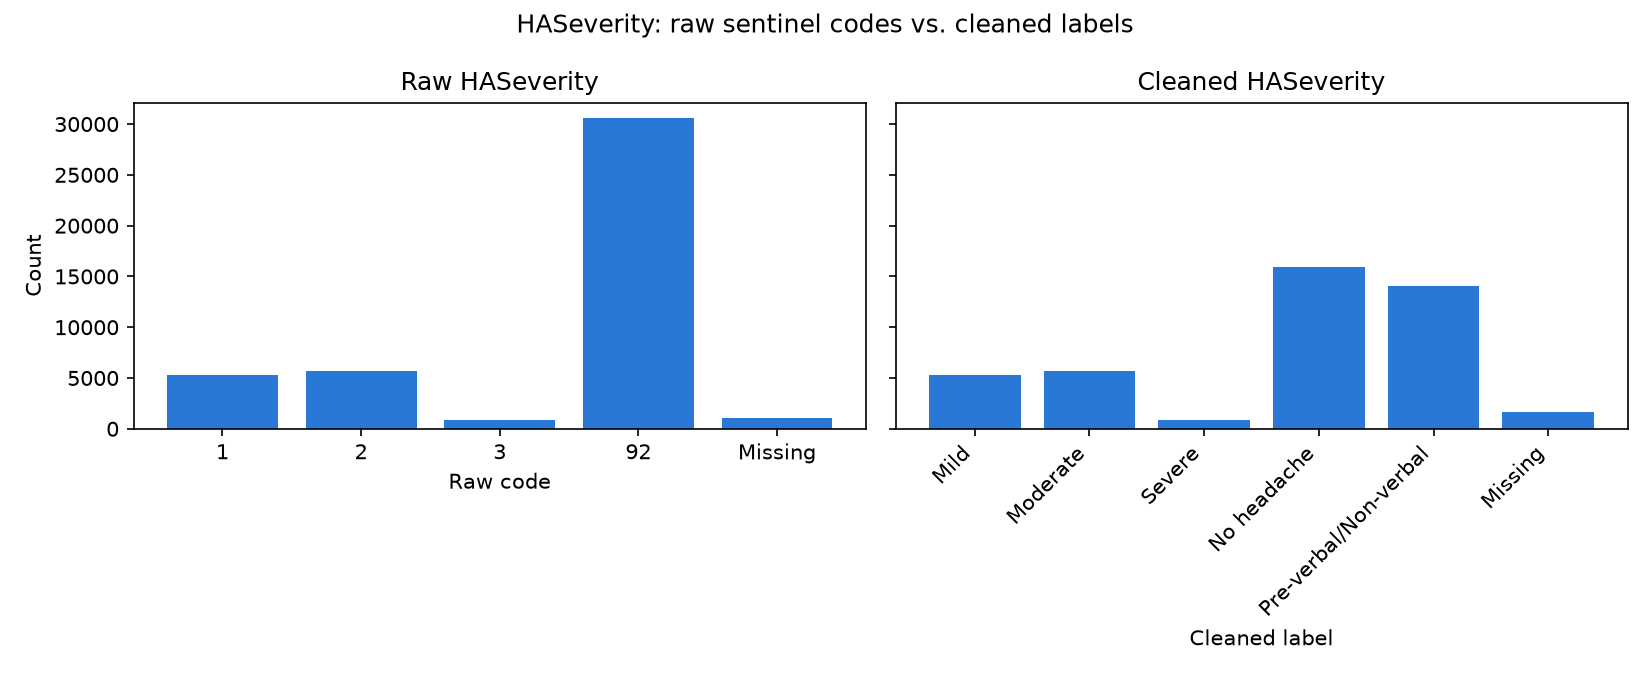
\includegraphics[width=0.87\textwidth]{../figs/haseverity_raw_vs_cleaned.png}
\caption{\texttt{HASeverity} collects headache severity and is the daughter variable to
\texttt{HA\_verb}, which collects headache presence, from the PECARN TBI dataset. The left panel
shows the headache severity raw integer codes. The right panel shows the corresponding cleaned
labels. The single raw sentinel value 92 represents two meaningfully different values:
``No headache'' versus ``Pre-verbal/Non-verbal.''}
\label{fig:haseverity}
\end{figure}

\texttt{clean.py} handles this information-loss issue for all variables with this family
structure. Specifically, the \texttt{clean\_gated\_family} and \texttt{clean\_gated\_detail}
functions implement the following: (1) if the parent variable indicates a real value, the
daughter's raw code maps to its real label term (not just integer coding); (2) if the parent's
answer has a specific coded meaning that isn't a real answer (e.g. ``No headache,''
``Pre-verbal/Non-verbal,'' ``CT not ordered''), the daughter variable is relabeled with that value;
(3) if the parent's answer is unknown, or if the parent variable value is real but the daughter
variable value is blank, then the value becomes a true NaN. I also added a
\texttt{clean\_gated\_family} wrapper function that applies this logic to an entire parent/daughter
group at once, so the parent variable's own value gets relabeled to the corresponding term, and
every daughter under it is processed consistently against the same rule. The parent variables
cleaned by this logic are: \texttt{HA\_verb}, \texttt{LOCSeparate}, \texttt{Seiz}, \texttt{Vomit},
\texttt{Hema}, \texttt{SFxBas}, \texttt{Clav}, \texttt{NeuroD}, \texttt{OSI}, \texttt{CTForm1},
\texttt{CTSed}, \texttt{AMS}, \texttt{SFxPalp}, \texttt{CTDone}.

Standalone variables were also relabeled so their values became similarly easily interpretable. These are
columns with no parent/daughter structure --- just a direct code-to-label mapping, cleaned
separately from the family logic. The standalone variables include: \texttt{ActNorm},
\texttt{Dizzy}, \texttt{Intubated}, \texttt{Paralyzed}, \texttt{Sedated}, \texttt{Amnesia\_verb},
\texttt{Race}, \texttt{Gender}, \texttt{Ethnicity}, \texttt{AgeTwoPlus}, \texttt{FontBulg},
\texttt{GCSGroup}, \texttt{Drugs}, \texttt{GCSEye}, \texttt{GCSVerbal}, \texttt{GCSMotor},
\texttt{EmplType}, \texttt{Certification}, \texttt{InjuryMech}, \texttt{High\_impact\_InjSev},
\texttt{Observed}, \texttt{EDDisposition}, \texttt{DeathTBI}, \texttt{HospHead},
\texttt{HospHeadPosCT}, \texttt{Intub24Head}, \texttt{Neurosurgery}, \texttt{PosIntFinal}.

Finally, \texttt{PatNum}, \texttt{GCSTotal}, \texttt{AgeInMonth}, and \texttt{AgeinYears} were left
untouched, as they are purely numeric/ID fields with no coding.

Following the main cleaning functions, I wanted to confirm this logic made sense. The
\texttt{verify\_gated\_cleaning} function checks two things per family: (1) each special label's
count was checked against how many rows actually had the specific parent-variable value that
produces that label, and (2) the NaN count was checked against the number of rows where the parent
variable's value didn't correspond to either a real answer or a special label, plus the number of
rows where the parent variable did indicate a real answer but the daughter's own raw value was
still missing. Every variable family checked passed with zero mismatches. This check is part of
\texttt{clean.py} but can be manually turned on and off with a verbose option.

\subsection{Data Exploration}\label{data-exploration}

Beginning data exploration, I was interested in variables that were not discussed thoroughly, or
at all, in the original paper (Kuppermann et al. 2009). Specifically, I wanted to further explore
the demographic and indication-for-CT-scan variables in the dataset and see how they correlate
with the domain question. The PECARN TBI dataset had demographic information on ethnicity, gender,
and race. Ethnicity showed a high proportion of missingness and relatively unbalanced data, making
it a poor candidate for further investigation (Fig. 2). Gender and race have much less missingness and more
balanced data (Fig. 3 and 4). Exploring the demographic data left me most interested in how race associates with
CT and TBI: gender showed no meaningful gap in CT or TBI, whereas race showed some interesting
differences that I explored further in Finding 1.

\begin{figure}[h]
\centering
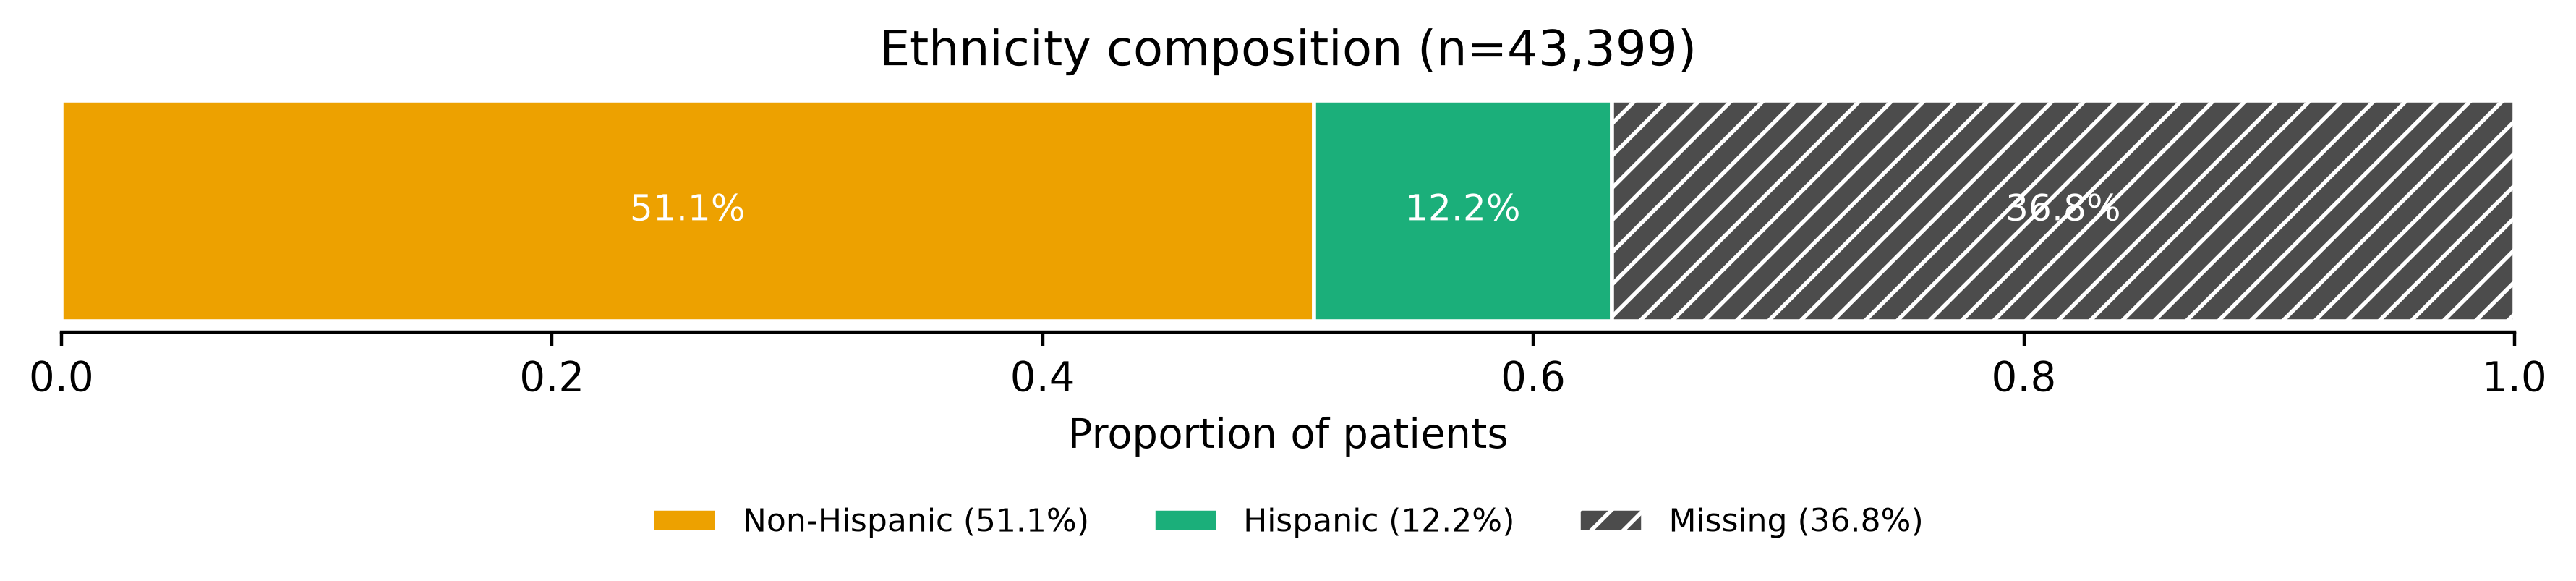
\includegraphics[width=\textwidth]{../figs/ethnicity_composition.png}
\caption{Ethnicity composition of the PECARN TBI dataset, showing how the data is classified as
Non-Hispanic, Hispanic, or Missing. Ethnicity has high missingness in this dataset.}
\label{fig:ethnicity}
\end{figure}

\begin{figure}[h]
\centering
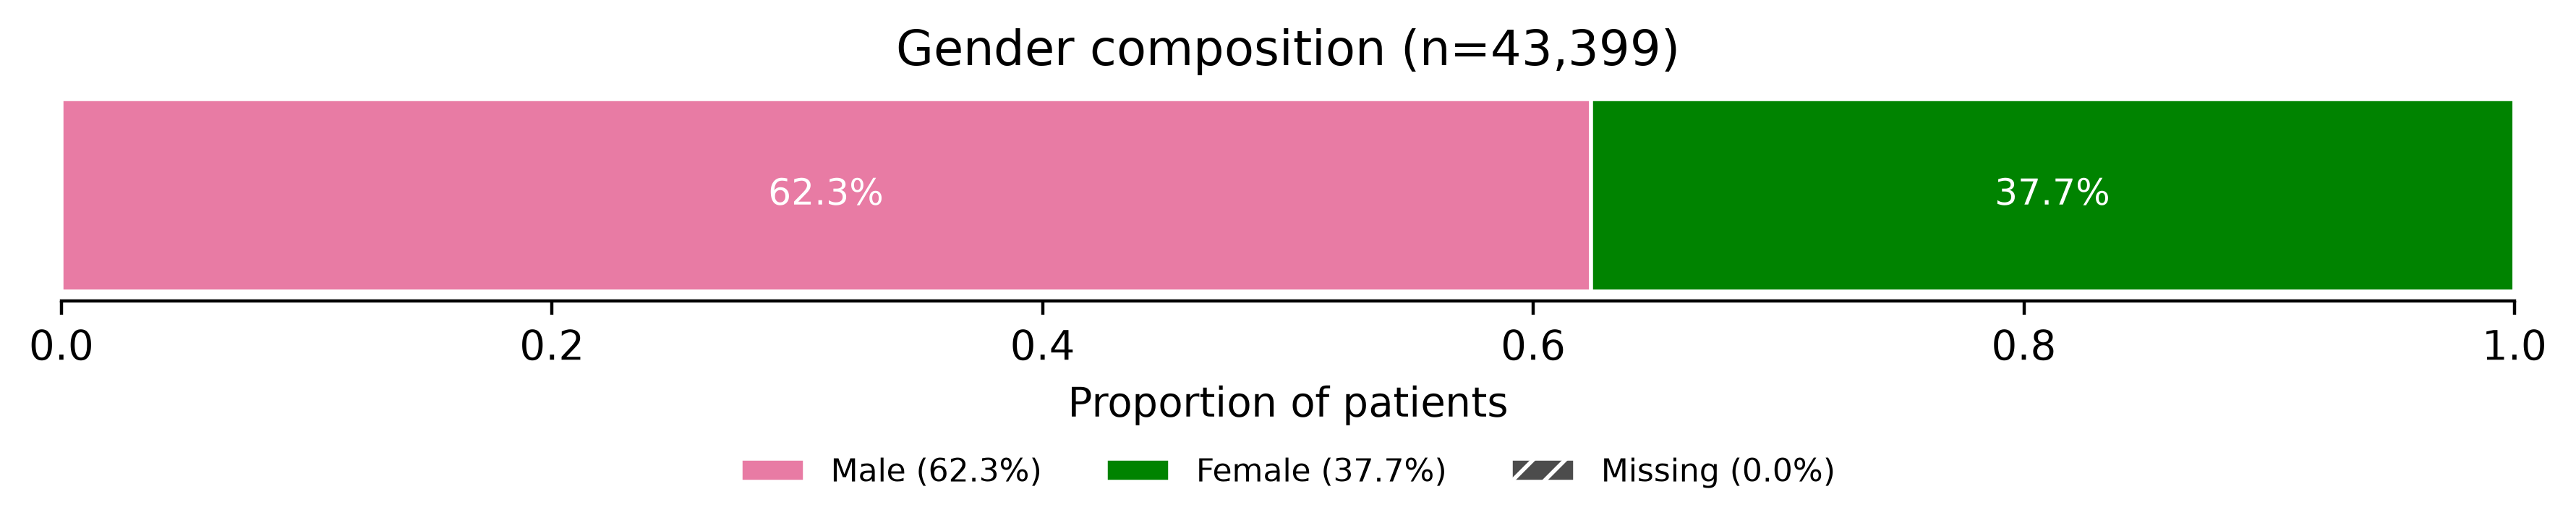
\includegraphics[width=\textwidth]{../figs/gender_composition.png}
\caption{Gender composition of the PECARN TBI dataset, showing how the data is classified as Male,
Female, or Missing. Gender has very low missingness in this dataset.}
\label{fig:gender}
\end{figure}

\begin{figure}[h]
\centering
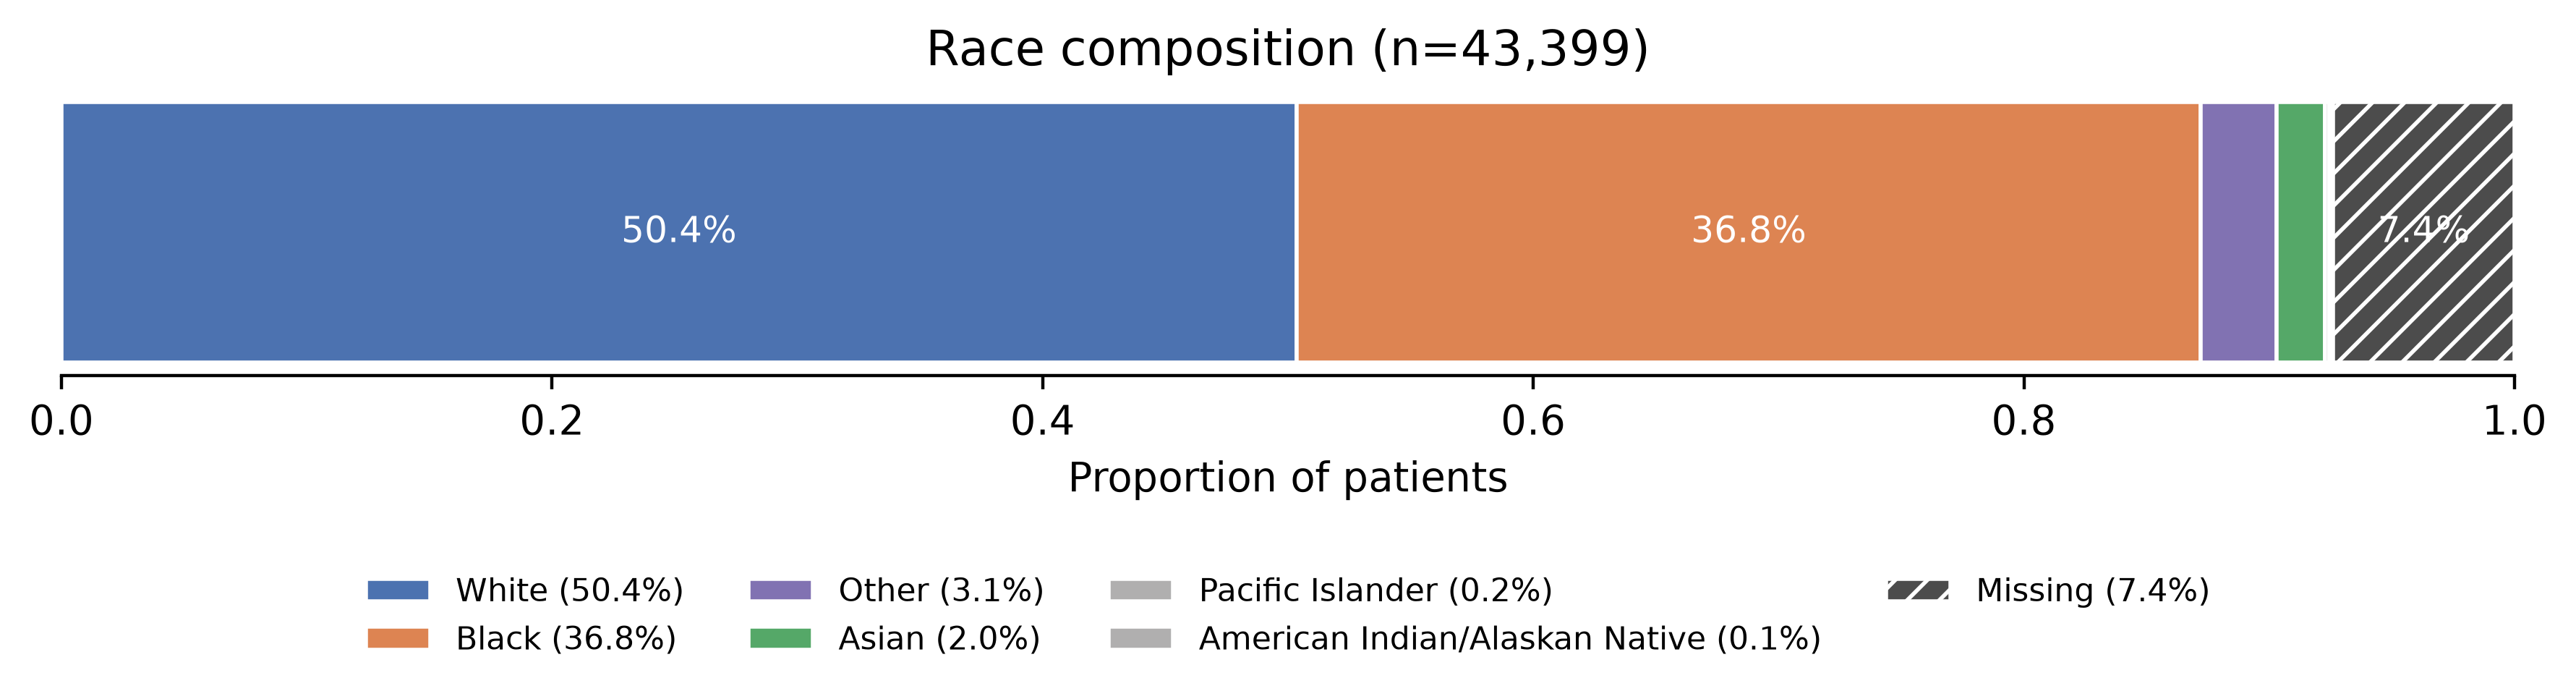
\includegraphics[width=\textwidth]{../figs/race_composition.png}
\caption{Race composition of the PECARN TBI dataset, showing how the data is classified as White,
Black, Other, Asian, Pacific Islander, American Indian/Alaskan Native, or missing. Race has low
missingness, as well as low counts for the Pacific Islander and American Indian/Alaskan Native
categories.}
\label{fig:race}
\end{figure}

Another variable I wanted to explore was indication for CT  (Fig. 5). Initial data exploration shows a
majority of patients are assigned more than two indications for a CT scan. Considering that most
patients are cited with more than two indications, I wanted to look at the types and frequency of
different indications across the dataset.

\begin{figure}[h]
\centering
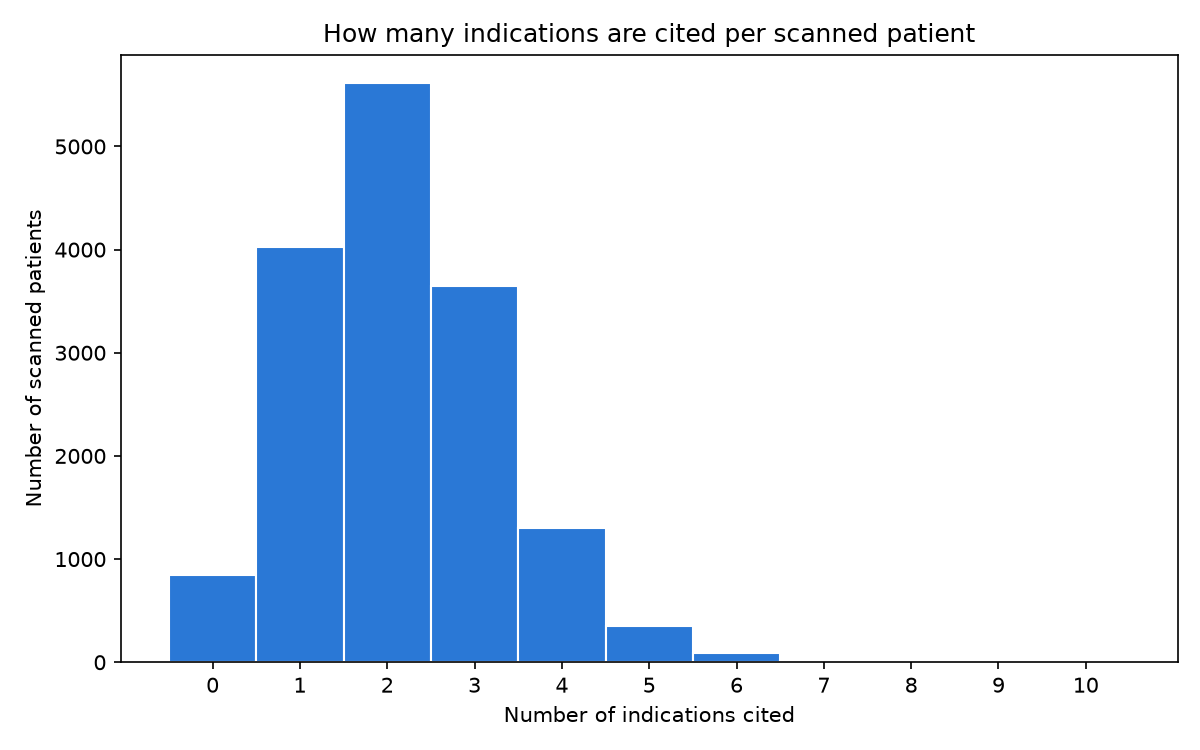
\includegraphics[width=0.48\textwidth]{../figs/indications_per_patient.png}\hfill
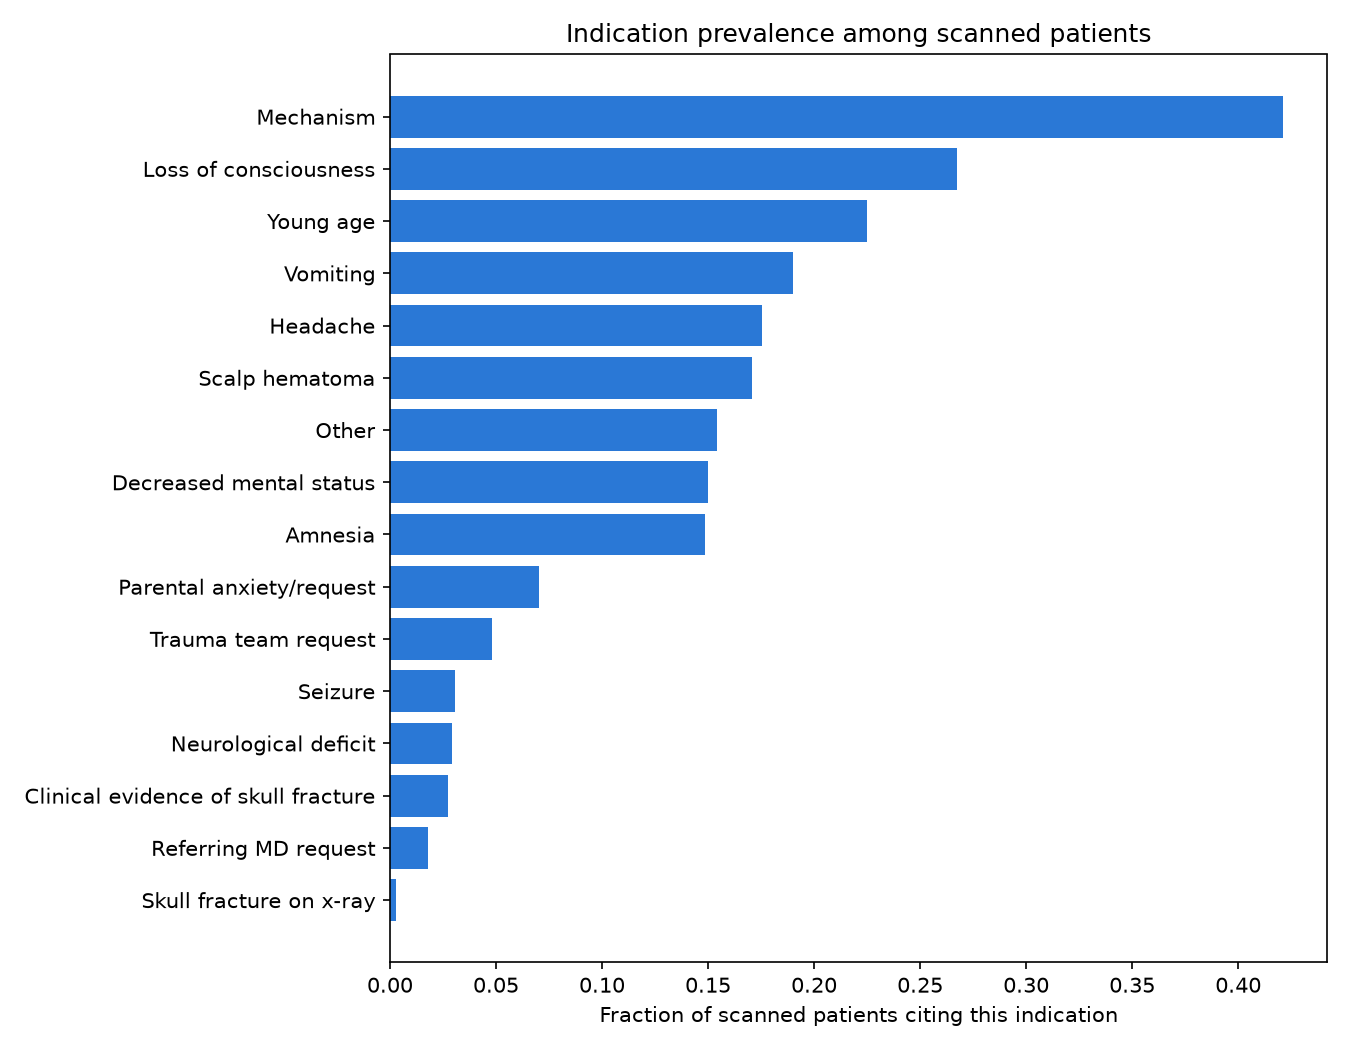
\includegraphics[width=0.42\textwidth]{../figs/indication_prevalence.png}
\caption{The left panel shows the number of indications cited for a CT scan. The right panel shows
the frequency of indication types cited. All from the PECARN TBI dataset.}
\label{fig:indications}
\end{figure}

\FloatBarrier

\section{Findings}\label{findings}

\subsection{First finding: CT utilization and yield by race}\label{first-finding}

To assess the association between race and CT/TBI outcomes, I looked at both utilization (who gets
scanned) and yield (whether scanning identified a ciTBI) across the three racial groups with
adequate sample sizes for interpretation. Black patients have both the lowest scan rate
($\sim$28\%, $n=4{,}523$ scanned) and the lowest yield (3.98\%), while White (42\% scan rate,
$n=9{,}307$ scanned; 4.80\% yield) and Asian (37\% scan rate, $n=321$ scanned; 5.31\% yield)
patients are higher on both measures (Fig. 6). In other words, utilization and yield move together across
these groups rather than trading off against each other: Black patients are scanned least and,
when scanned, least likely to actually have a ciTBI, while White and Asian patients are scanned
more liberally and still scan more accurately, so lower CT use for Black patients is not being
offset by better targeting of who gets scanned.

For this analysis, American Indian/Alaskan Native and Pacific Islander groups were excluded, as
the sample size was too small ($n=64/78$ scanned) to interpret and draw meaningful conclusions
from. It is also important to note that this is strictly associational, not causal, the current
analysis does not control for site, historical cohort ($\sim$2004--2006), or race as recorded in
the study rather than self-identified, all of which could be influential on the findings.

\begin{figure}[h]
\centering
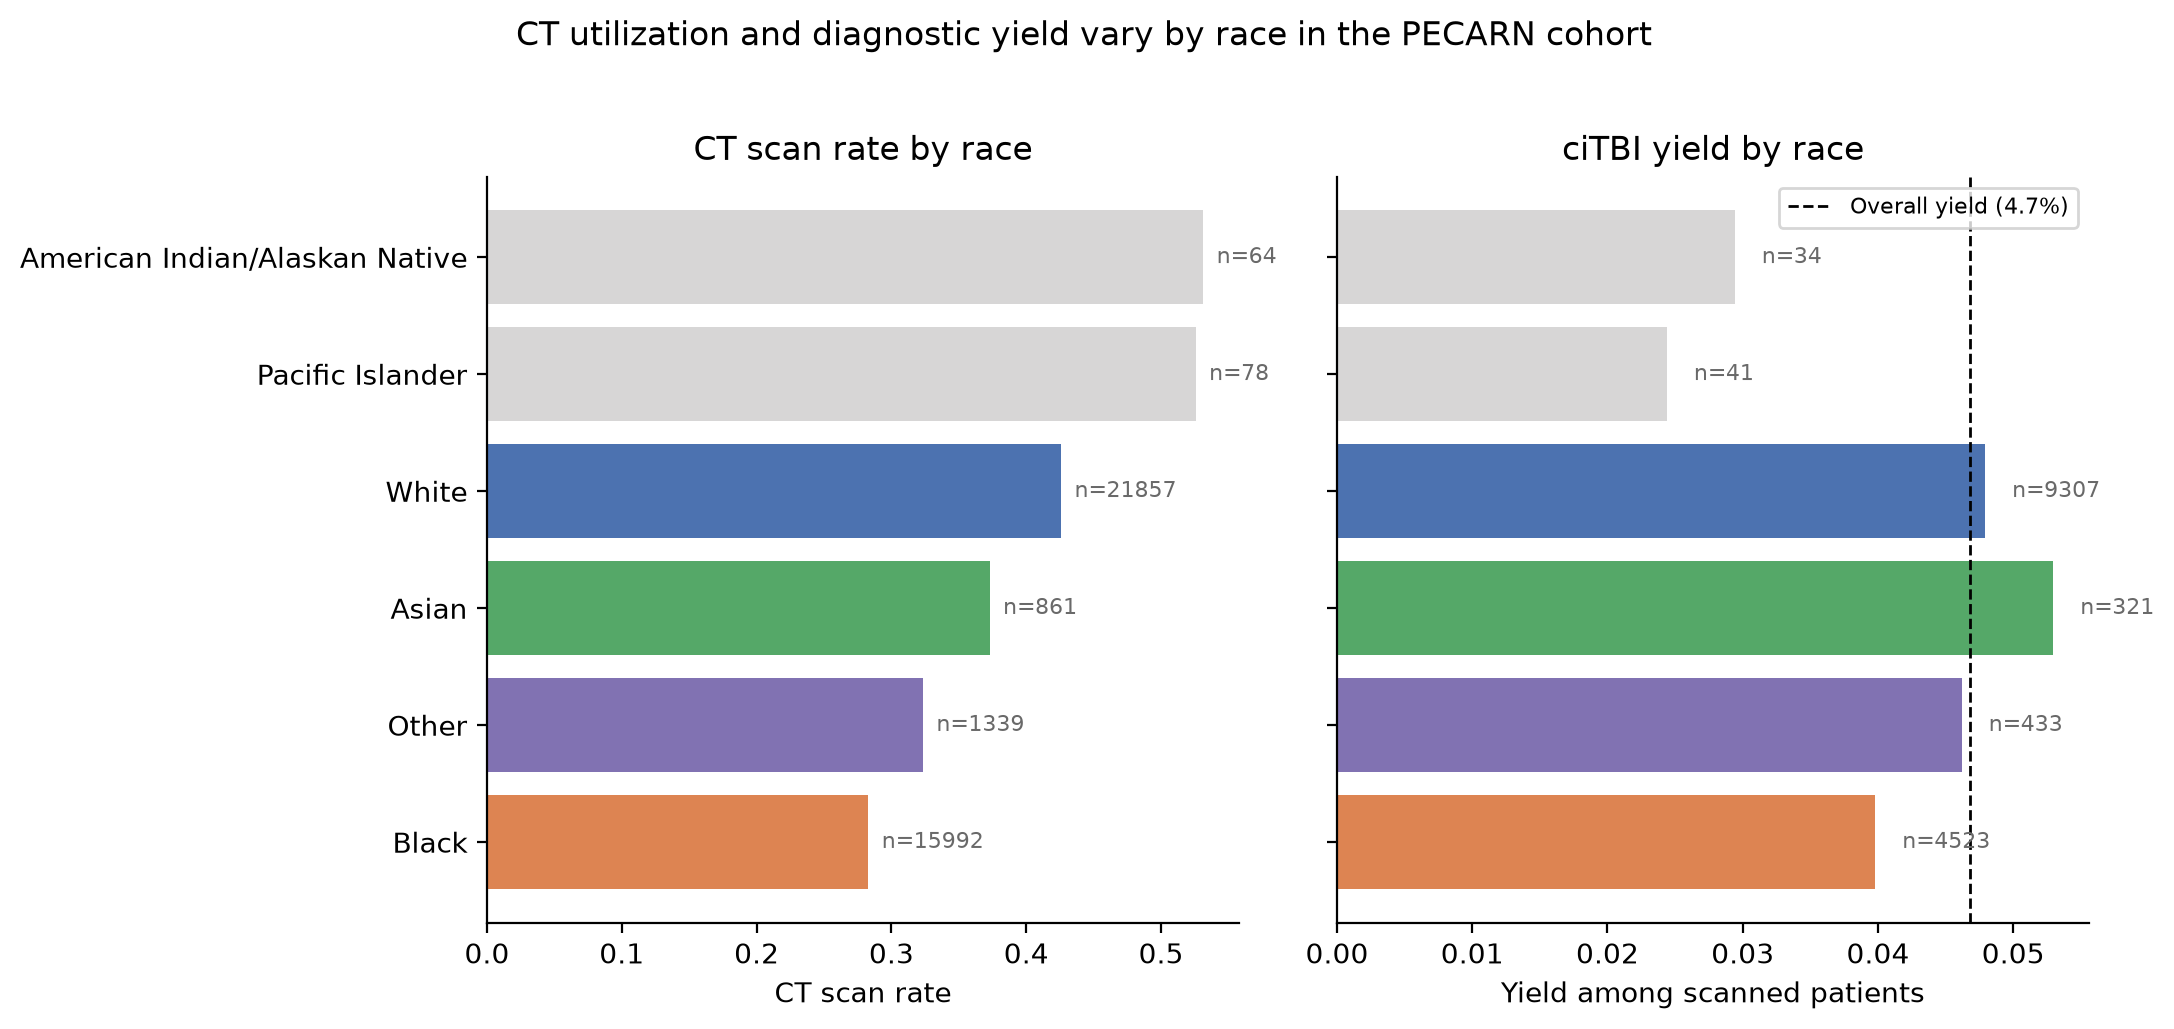
\includegraphics[width=\textwidth]{../figs/race_ct_yield.png}
\caption{CT utilization and diagnostic yield by race in the PECARN TBI cohort. The left panel shows
the fraction of all patients in a specified race group who got scanned, regardless of outcome. The
right panel shows the proportion of CT-scanned patients who had ciTBI, compared to the overall
yield.}
\label{fig:ct-race}
\end{figure}

\subsection{Second finding: Indication yield}\label{second-finding}

To identify which of the 16 clinical indications for CT are actually predictive of injury rather
than just commonly cited, I computed yield (the fraction of scanned patients
($\texttt{CTDone}=1$) with a positive CT and the fraction with a confirmed ciTBI) for each
indication, excluding \texttt{IndXraySFx} for small $n$ (Fig. 7). This analysis revealed a clear hierarchy:
clinical evidence of skull fracture is the single strongest indication by a wide margin
($\sim$38\% positive CT, $\sim$27\% ciTBI, $n=438$), followed by neurological deficit
($\sim$18\%/17\%, $n=462$) and decreased mental status ($\sim$17\%/15\%, $n=2{,}382$), both of
which track closely between positive CT and ciTBI rather than showing the wide gap seen elsewhere
in the chart. By contrast, the highest-volume indications, mechanism ($\sim$10\%/7\%,
$n=6{,}694$), loss of consciousness ($\sim$8\%/6\%, $n=4{,}250$), and vomiting ($\sim$7\%/5\%,
$n=3{,}025$), are right around the overall-yield reference lines, meaning they're commonly cited
but only modestly discriminating. The clearest anomaly is among the ``request-driven''
indications: trauma team request behaves like a genuine clinical indicator ($\sim$13\%/12\%,
$n=766$), well above the reference lines, whereas referring MD request ($\sim$6\%/3\%, $n=282$) and
parental anxiety/request ($\sim$2\%/1\%, $n=1{,}115$) fall near the bottom of the ranking, so a
scan being requested is not by itself informative, but a scan requested specifically by the trauma
team is. Headache and parental anxiety/request are the two lowest-yield indications overall, acting as
 reassurance scans rather than indications with real diagnostic information. 

\begin{figure}[h]
\centering
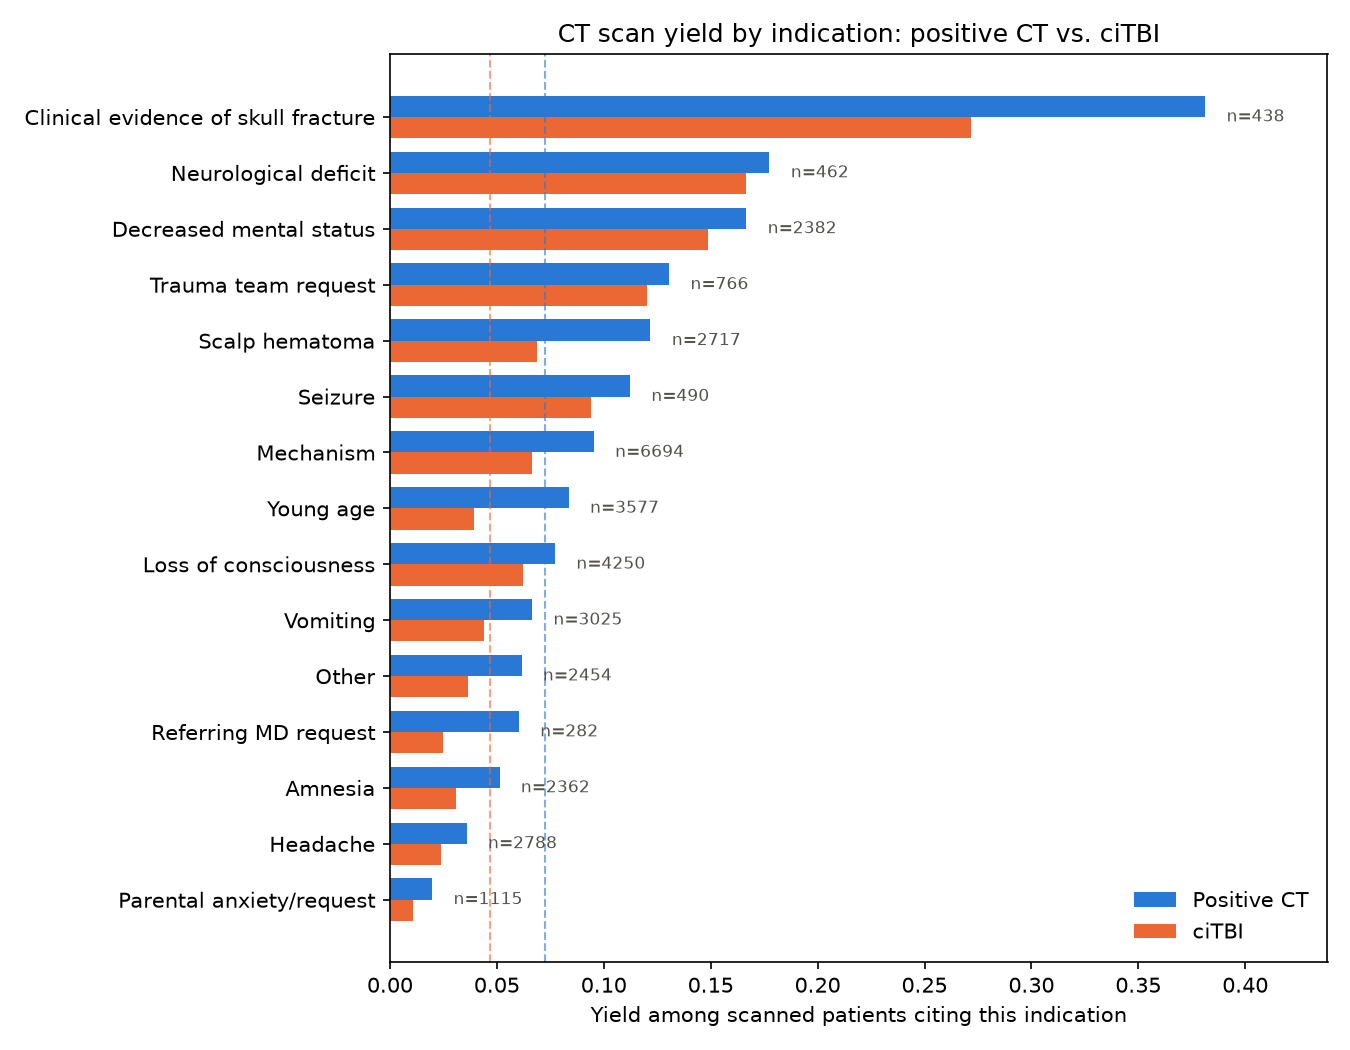
\includegraphics[width=\textwidth]{../figs/indication_yield.png}
\caption{CT scan yield by indication for both positive CT (PosCT) and ciTBI, compared to average
lines. The orange dashed line is the overall ciTBI yield across all indications combined, and the
blue dashed line is the overall positive-CT yield across all indications combined.}
\label{fig:indication-yield}
\end{figure}

\subsection{Reality Check}\label{reality-check}

A natural reality check for this dataset is the original PECARN study itself: Kuppermann et al.
(2009) report descriptive statistics for the same cohort in a peer-reviewed publication, which
provides an external, independent benchmark rather than a subjective judgment of whether the cleaned
numbers ``look right.'' If the cleaned data reproduce the paper's headline figures, that is strong
evidence that our cleaning and derived-variable logic are correct.

The first attempt at this comparison did not match. The fully cleaned dataset contains
$n = 43{,}399$ patients, versus the paper's analytic sample of $n = 42{,}412$. More concerning, several key rates ran consistently high relative to the paper: the
CT rate, the rate of TBI-on-CT among scanned patients, the overall ciTBI rate, and especially the
rate of neurosurgery among ciTBI cases (Table \ref{tab:reality-check-initial}). The
neurosurgery-among-ciTBI rate in particular was off by more than 10 percentage points, which was
too large a gap to attribute to rounding or minor coding differences.

\begin{table}[h]
\centering
\caption{Cleaned dataset vs. Kuppermann et al. (2009), full sample}
\label{tab:reality-check-initial}
\begin{tabular}{lrrr}
\toprule
Metric & Paper (Kuppermann 2009) & Cleaned dataset & Abs. difference \\
\midrule
Total N & 42412 & 43399 & 987 \\
CT rate (\%) & 35.3 & 36.63 & 1.33 \\
TBI-on-CT rate among scanned (\%) & 5.2 & 7.27 & 2.07 \\
ciTBI rate overall (\%) & 0.9 & 1.76 & 0.86 \\
Neurosurgery rate among ciTBI (\%) & 15.9 & 26.21 & 10.31 \\
Hospital admission rate (\%) & 9.0 & 2.0 & $-7.0$ \\
\bottomrule
\end{tabular}
\end{table}

This discrepancy was due to the reality check being done on the dataset before the exclusion criteria in the paper were applied (excluded patients with a GCS score of 3--13, retaining only patients with GCS 14--15). 

We tested this by restricting the cleaned data to $\texttt{GCSTotal} \in \{14, 15\}$ and
dropping rows with missing outcome data. This restriction brought the sample size to 
$n = 42{,}412$, matching the paper's analytic sample size, and the rates checked previously began to agree with the published values (Table
\ref{tab:reality-check-restricted}). Most strikingly, our GCS 14--15 subset reproduces the paper's
exact reported count of 376 ciTBI cases.

\begin{table}[h]
\centering
\caption{Cleaned dataset (GCS 14--15 subset) vs. Kuppermann et al. (2009)}
\label{tab:reality-check-restricted}
\begin{tabular}{lrrr}
\toprule
Metric & Paper (Kuppermann 2009) & Cleaned dataset (GCS 14--15) & Abs. difference \\
\midrule
Total N & 42412 & 42412 & 0 \\
CT rate (\%) & 35.3 & 35.3 & 0.0 \\
TBI-on-CT rate among scanned (\%) & 5.2 & 5.2 & 0.0 \\
ciTBI rate overall (\%) & 0.9 & 0.89 & 0.01 \\
ciTBI count & 376 & 376 & 0 \\
Neurosurgery rate among ciTBI (\%) & 15.9 & 16.0 & 0.1 \\
\bottomrule
\end{tabular}
\end{table}

\subsection{Stability Check}\label{stability-check}


As a sanity check on injury-mechanism severity as a possible confound, the severity-mix chart shows
that the mechanism-severity distribution (Low/Moderate/High) is broadly similar across race, with
Black patients showing a slightly lower high-severity share (13.6\%) than White (16.2\%) or Asian
(17.1\%) patients (Fig. 8). 

\begin{figure}[h]
\centering
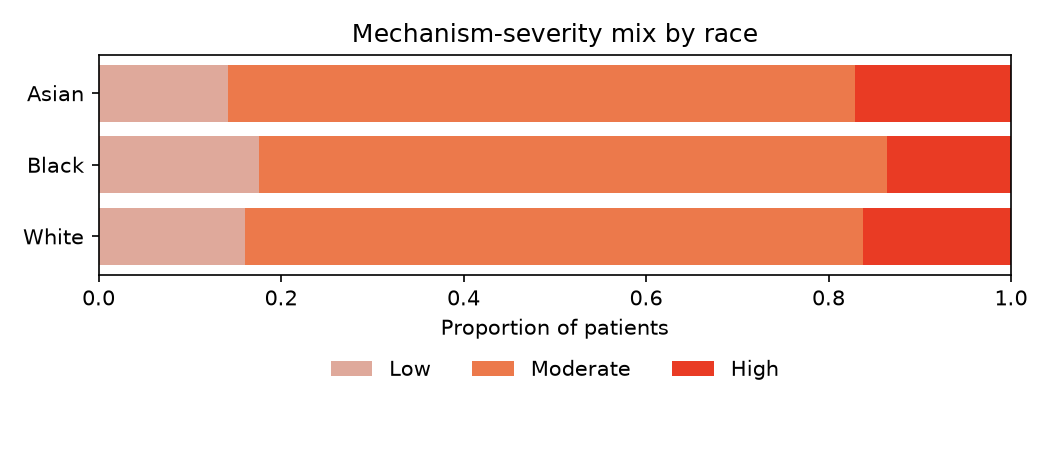
\includegraphics[width=\textwidth]{../figs/severity_mix_by_race.png}
\caption{Injury mechanism severity proportions compared across Asian, Black, and White patients.}
\label{fig:severity-mix}
\end{figure}

The before-and-after comparison is given by the aggregate and stratified yield charts (Fig 9 and 10). Before
stratifying, the aggregate ciTBI yield is higher for White patients (4.79\%, $n=9{,}307$) than
Black patients (3.97\%, $n=4{,}523$). After stratifying by mechanism severity, this gap holds up
within the two best-powered strata: Moderate severity (White 3.95\%, $n=6{,}081$ vs. Black 2.83\%,
$n=2{,}831$) and High severity (White 9.29\%, $n=1{,}982$ vs. Black 8.14\%, $n=1{,}059$). It only
reverses in the smallest, noisiest stratum, Low severity (White 1.31\%, $n=1{,}150$ vs. Black
1.40\%, $n=570$), where the sample size is small enough that this reversal should not be read as
meaningful.

\begin{figure}[h]
\centering
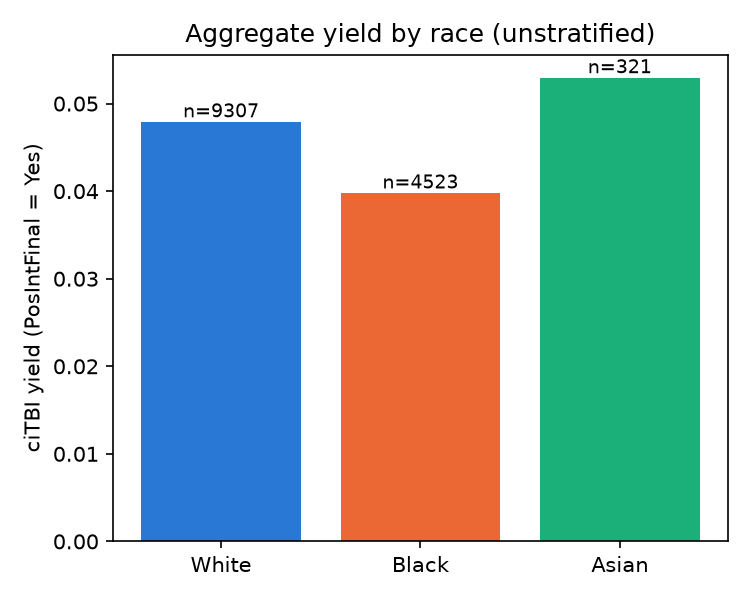
\includegraphics[width=0.77\textwidth]{../figs/before_race_yield.png}
\caption{ciTBI yield aggregated by race, before stratification by injury mechanism severity.}
\label{fig:yield-before}
\end{figure}

\begin{figure}[h]
\centering
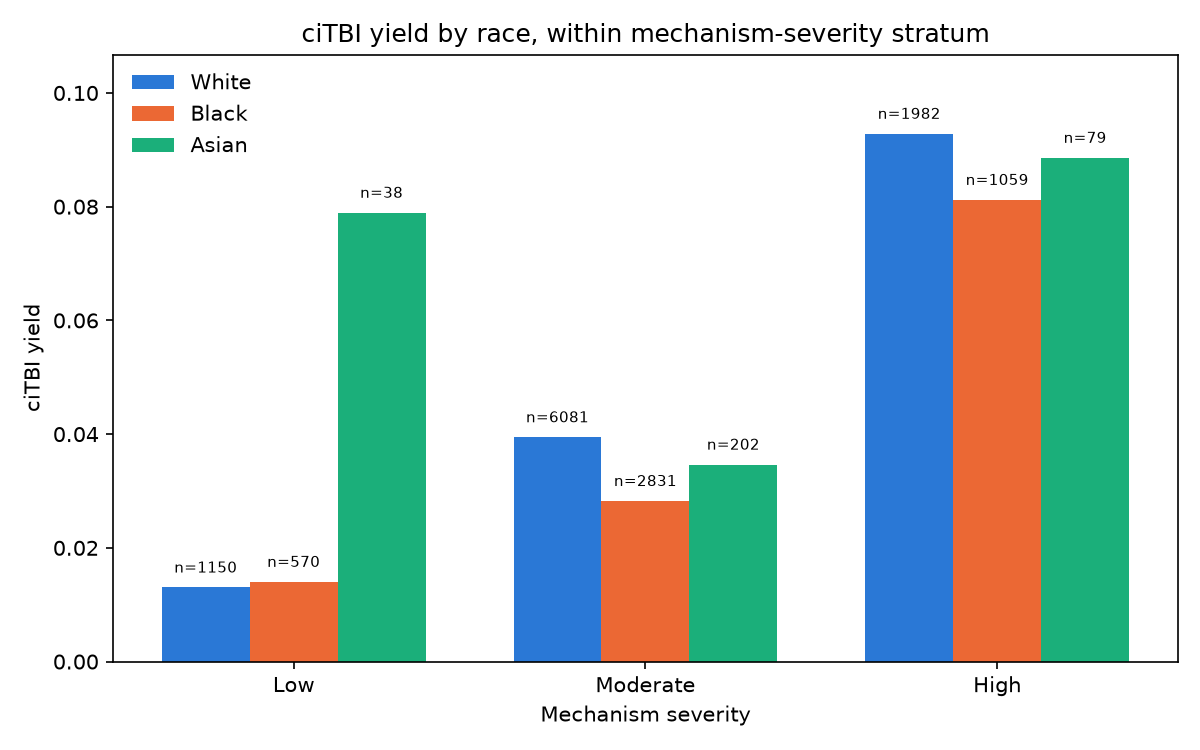
\includegraphics[width=\textwidth]{../figs/yield_by_race_and_severity.png}
\caption{ciTBI yield aggregated by race, after stratification by injury mechanism severity.}
\label{fig:yield-after}
\end{figure}

Taken together, this is evidence that the race/yield gap is not simply an artifact of differing
injury severity across groups. It survives a direct confounding variable check available with this
data.

\section{Modeling}

\subsection{Implementation}

To predict clinically important traumatic brain injury (ciTBI, \texttt{PosIntFinal}), I restricted the model to four pre-CT predictors --- \texttt{LOCSeparate}, \texttt{AMS}, \texttt{Vomit}, and \texttt{HA\_verb} --- selected because they are observable during the initial clinical evaluation, before a CT scan is ordered. This constraint reflects that a decision rule is only useful if it can guide the imaging decision itself, so it cannot rely on information obtained from the CT. Rows with missing values on any of these four variables were dropped rather than imputed, keeping the modeling sample restricted to complete cases. Categorical predictors were one-hot encoded with the reference level dropped to avoid collinearity in the design matrix. The data were then split into training and test sets using a 75/25 split, stratified on the outcome to preserve ciTBI's low prevalence in both subsets, with \texttt{random\_state=0} set for reproducibility.

We fit a logistic regression with scikit-learn's default $L_2$ regularization and a decision tree constrained to \texttt{max\_depth=4}. The tree depth was set manually to keep the resulting tree small enough to draw and trace by hand. This judgment call reflects the domain problem's emphasis on ease of use. On the test set, the logistic regression achieved an AUC of 0.876, slightly outperforming the decision tree's AUC of 0.864, suggesting that the added interpretability and simplicity of the shallow tree came at only a small cost in discriminative performance.

\subsection{Stability}

As a stability check, I revisited the mechanism-severity perturbation from Section~\ref{stability-check}, this time adding Low/Moderate/High severity as a control feature to both models rather than stratifying the data by it. Both models improved: logistic regression's test AUC rose from 0.876 to 0.914, and the decision tree's from 0.864 to 0.897. This stands in contrast to the race/yield finding in Section~\ref{stability-check}, where controlling for severity left the conclusion essentially unchanged, indicating severity was not a confound driving that result. Here, the improvement in both models shows severity is not merely a nuisance variable to control away but an independently predictive feature, consistent with the domain intuition that higher-energy mechanisms inflict more physical injury on top of whatever the four clinical signs already capture.

The logistic regression's coefficients show a clean, monotonic ordering relative to the dropped ``High'' reference: Low severity carries a coefficient of $-2.15$ and Moderate $-1.02$, so estimated risk rises steadily as severity moves from Low to Moderate to High. The decision tree shows a similar picture through a different mechanism: Low severity has a feature importance of 0.072 that ranks above both Vomit = Yes and LOCSeparate = Suspected, while Moderate severity's importance is essentially zero ($\approx 0.0004$) and is largely unused. Both models mainly learn to carve out Low severity as a distinctly lower-risk group, without cleanly separating Moderate from High. The two analyses point to the same conclusion from different angles: Low severity behaves like a distinct risk group, both in the original stratified finding and in how the predictive models treat it as a feature.

\begin{figure}[h]
\centering
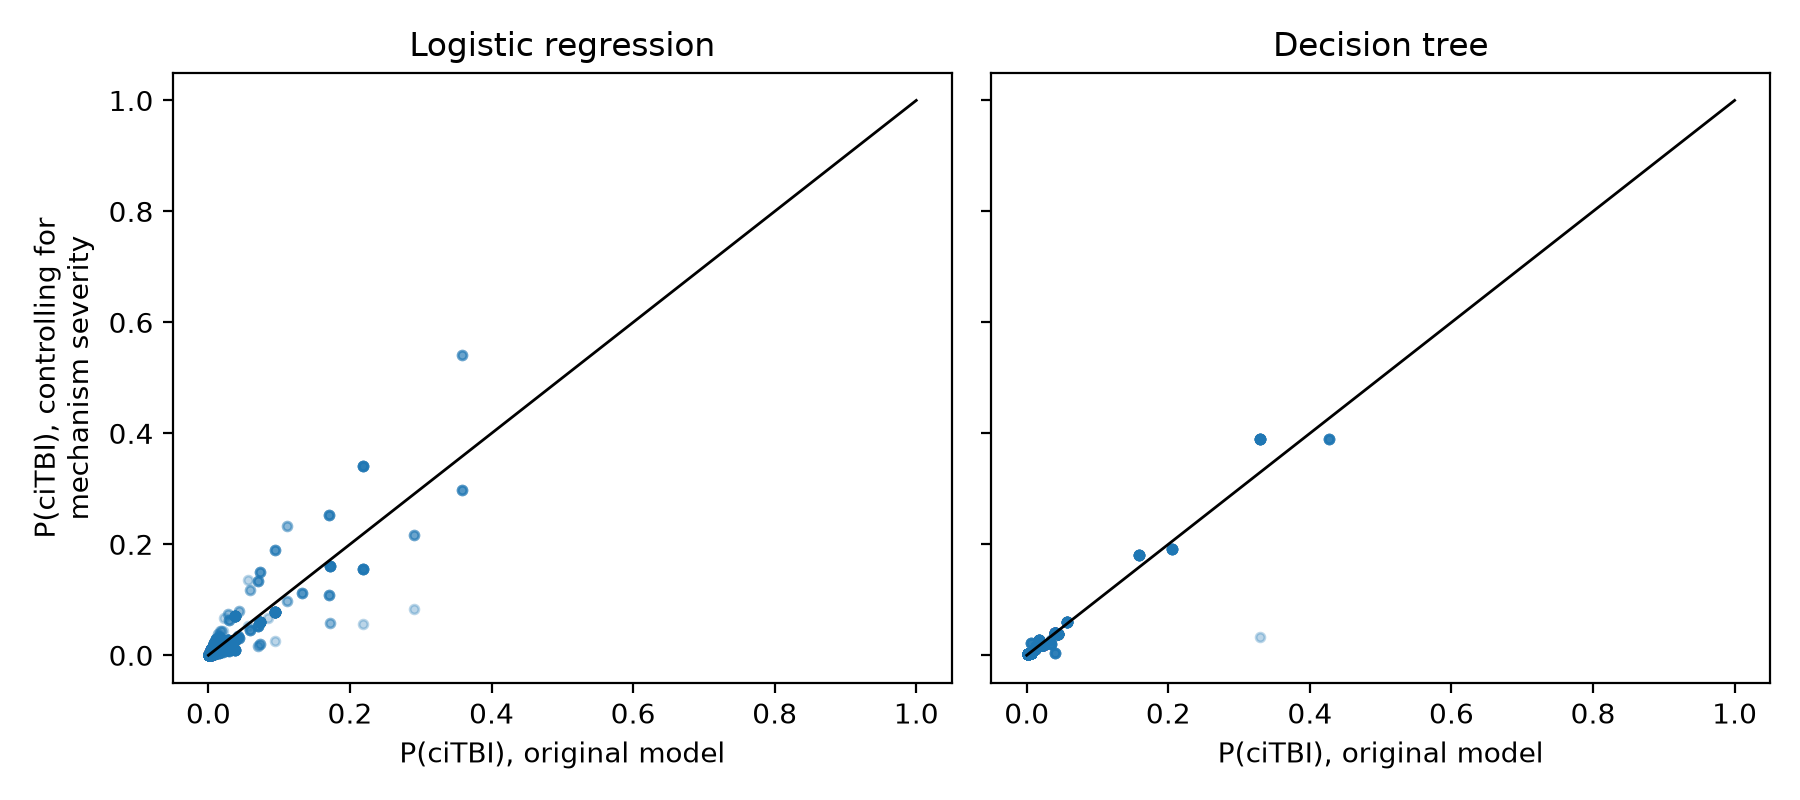
\includegraphics[width=\textwidth]{../figs/stability_severity_control.png}
\caption{Predicted probability of ciTBI on the test set from each model before vs.\ after controlling for injury-mechanism severity, with the $y=x$ line shown for reference.}
\label{fig:model-stability}
\end{figure}

\subsection{Discussion}

I chose these two models because logistic regression assumes the four predictors combine additively on the log-odds scale, while a decision tree can capture interactions and nonlinear thresholds. A large AUC gap between the two would therefore be diagnostic, signaling that the relationships among \texttt{LOCSeparate}, \texttt{AMS}, \texttt{Vomit}, and \texttt{HA\_verb} involve meaningful interaction or threshold effects that an additive model misses. In practice, no such gap appeared: the logistic regression's test AUC of 0.876 was very similar to the tree's AUC of 0.864. This suggests that most of the predictive signal carried by these four variables lives in their main effects rather than in interactions between them. Practically, that means a simple additive scoring rule, in the spirit of the actual PECARN rule, is not leaving much on the table here.

The logistic regression's interpretability comes from its additive structure, where exponentiating each coefficient gives an odds ratio directly interpretable by clinicians. The decision tree offers a different form of interpretability: because it is capped at \texttt{max\_depth=4}, it can be read directly as a flowchart of at most four sequential yes/no questions.

\section{Conclusion}\label{conclusion}

With 125 raw columns, it wasn't possible to visualize or inspect every variable and every pairwise relationship individually, so the choices of what to examine for the two Findings explored in EDA and the four modeling variables, were driven by domain reasoning rather than an exhaustive survey of the full column set. This dataset is human-collected clinical data, with sentinel missing-value codes (90/91/92) that required  the codebook variable by variable, along with judgment calls about when a code meant ``not applicable'' versus genuinely missing. Therefore the this analysis reflects clinicians' data-entry decisions and PECARN's coding scheme as much as it reflects the underlying injuries themselves. Finally, there is no clean one-to-one correspondence between these variables and the reality they're meant to capture: AMS and ``suspected'' loss of consciousness are clinician judgment calls rather than objective measurements, and a verbal history of headache depends on patient or caregiver recall, but the documentation spreadsheet is what allowed us to make transparent, principled decisions about those gaps rather than guessing. 
Looking ahead, its worth noting PECARN is a single research network from one era of clinical practice, and needs external validation on an independent cohort collected at a different hospital system or in a later era of clinical practice.

\section{Academic honesty statement}\label{academic-honesty-statement}

Dear Bin,

I affirm that the work in this report is my own, and that all sources I used, including any discussions with classmates, are properly cited. Academic research honesty is necessary as it is the foundation of trust in science and the integrity of the field at large. Not only do we as researchers have an obligation to be honest to ourselves, our labs, and the greater scientific community when it comes to research, but also to the public, as many of us are funded by tax dollars and want our findings to be helpful to humanity.

\section{Collaborators}\label{collaborators}

Not Applicable.

\section{Bibliography}\label{bibliography}

Kuppermann N, Holmes JF, Dayan PS, Hoyle JD, Atabaki SM, Holubkov R, Nadel FM, Monroe D, Stanley RM,
Borgialli DA, Badawy MK, Schunk JE, Quayle KS, Mahajan P, Lichenstein R, Lillis KA, Tunik MG, Jacobs
ES, Callahan JM, Gorelick MH, Glass TF, Lee LK, Bachman MC, Cooper A, Powell EC, Gerardi MJ, Melville
KA, Muizelaar JP, Wisner DH, Zuspan SJ, Dean JM, Wooten-Gorges SL, for the Pediatric Emergency Care
Applied Research Network (PECARN). Identifying children at very low risk of clinically-important
traumatic brain injuries after blunt head trauma. \emph{Lancet} 2009; 374: 1160--70.

\end{document}
